\documentclass[UTF8,a4paper,11pt,fontset=fandol]{ctexart}
\usepackage[margin=22mm,headheight=15pt]{geometry}
\usepackage{amsmath,booktabs,graphicx,xcolor,fancyhdr,caption}
\usepackage[hidelinks]{hyperref}

\definecolor{ink}{HTML}{16324F}
\definecolor{secondary}{HTML}{4B5B69}
\ctexset{section={format=\Large\bfseries\color{ink},beforeskip=1.25ex,afterskip=0.95ex}}
\captionsetup{font=small,labelfont=bf,skip=5pt,hypcap=false}
\hypersetup{pdftitle={Vita01evt 地形牵引力实验}}
\setlength{\parindent}{0pt}
\setlength{\parskip}{5pt}
\renewcommand{\arraystretch}{1.18}
\pagestyle{fancy}
\fancyhf{}
\fancyhead[L]{\small\color{secondary}Vita01evt 地形牵引力实验}
\fancyhead[R]{\small\color{secondary}2026 年 11 月 16 日}
\fancyfoot[C]{\small\color{secondary}\thepage}
\renewcommand{\headrulewidth}{0.35pt}
\newcommand{\unit}[1]{\,\mathrm{#1}}

\begin{document}
{\LARGE\bfseries\color{ink}Vita01evt 地形牵引力实验\par}
{\color{secondary}MuJoCo 4.0.1 \quad \texttt{model\_10000} \quad 2026 年 11 月 16 日\par}

\section*{施力设置}

三组实验均使用开启速度跟踪奖励的同一策略。取世界系 \(+x\) 为试验前进方向，\(+z\) 竖直向上，\(\alpha\) 为绳子相对世界水平面的仰角。实验一和实验二的施力阶段，绳张力 \(F\) 与绳角 \(\alpha\) 均保持为该档的设定值。因此，世界系外力为
\[
  \mathbf F_w=(F\cos\alpha,\ 0,\ F\sin\alpha).
\]

牵引点固定在机身原点前方 \(17.287\unit{cm}\)，其机身系坐标为 \((0.17287,0,0)\unit{m}\)。牵引点随机器人移动和转动。在实验一和实验二中，机器人俯仰或改变航向时，换算到机身坐标系中的力方向随姿态改变。图中 \(\beta\) 为示意姿态的俯仰角，\(\gamma=\alpha-\beta\) 为矢状面内拉力与机身前向轴的夹角。

\begin{minipage}{\linewidth}
\centering
\makebox[\linewidth][c]{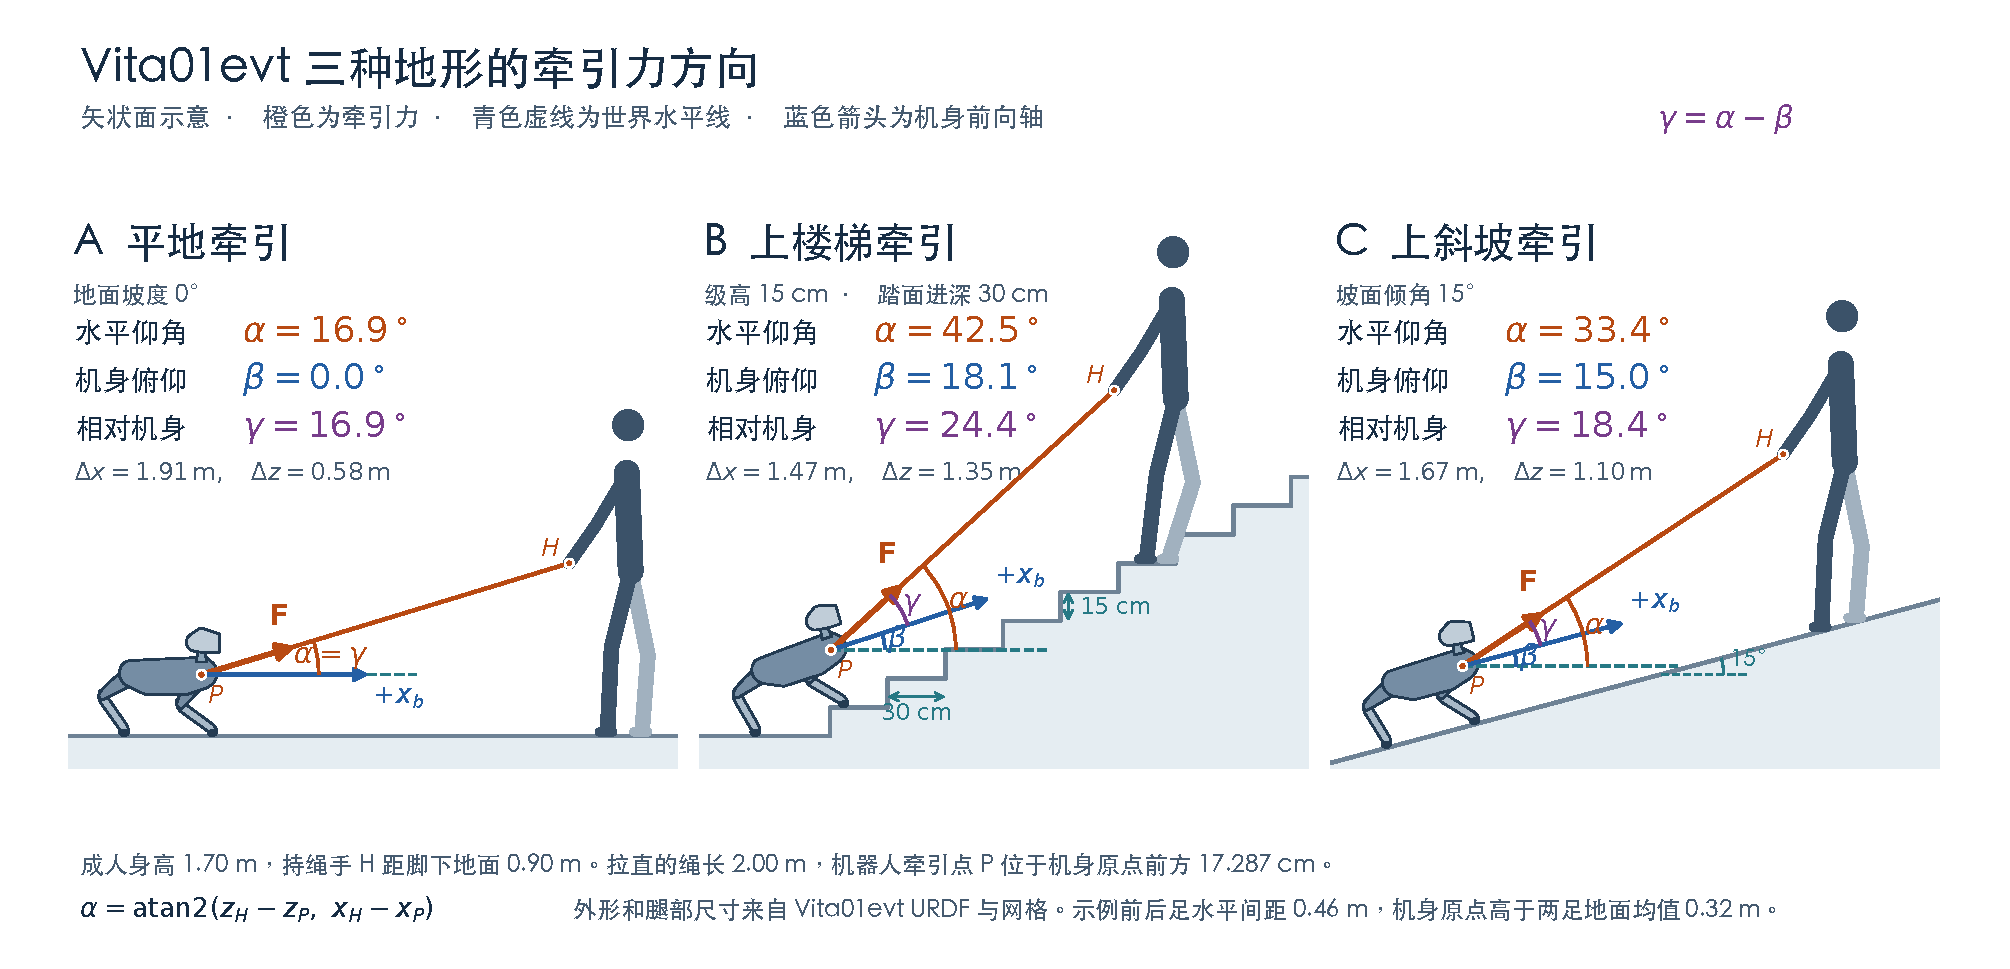
\includegraphics[width=176mm]{figures/traction_terrain_geometry.pdf}}
\captionof{figure}{实验一的三种牵引场景与预设绳角。橙色箭头表示施力方向，虚线表示世界水平面。}
\label{fig:rope-geometry}
\end{minipage}

实验一按图~\ref{fig:rope-geometry} 设置绳角，平地为 \(16.9^\circ\)，上坡为 \(33.4^\circ\)，上楼梯为 \(42.5^\circ\)。实验二对三种地形统一使用 \(33.4^\circ\)，以比较坡度与楼梯级高变化时所需的拉力。实验三固定矢状面内拉力相对机身的角度，按机身俯仰更新世界系绳角，见第~\ref{sec:body-angle} 节。

每个拉力档用五个初始位置复测。进入地形后，在世界系水平前向 \(x=1.2\) 至 \(3.6\unit{m}\) 的测量段内，用水平位移除以通过时间计算平均速度。

\clearpage
\section{三种地形达到相近速度所需的拉力}

本实验共 545 次，按图~\ref{fig:rope-geometry} 给定各地形的绳角。
斜坡坡度为 \(15^\circ\)，楼梯级高 \(15\unit{cm}\)，踏面深度 \(30\unit{cm}\)。

\begin{minipage}{\linewidth}
\centering
\captionof{table}{三种地形达到约 \(1.0\unit{m/s}\) 的实测拉力}
\begin{tabular}{l r c r}
\toprule
地形 & 绳张力 \(\mathrm{(N)}\) & 五次速度范围 \(\mathrm{(m/s)}\) & 相比平地 \(\mathrm{(N)}\) \\
\midrule
平地 & 21.80 & \(1.000\)--\(1.013\) & 基准 \\
\(15^\circ\) 斜坡 & 23.25 & \(0.996\)--\(1.013\) & \(+1.45\) \\
\(15\unit{cm}\) 楼梯 & 25.00 & \(0.956\)--\(1.007\) & \(+3.20\) \\
\bottomrule
\end{tabular}
\end{minipage}

平地在 \(30\unit{N}\) 下的速度中位数为 \(1.46\unit{m/s}\)，斜坡在 \(32\unit{N}\) 时测得相近中位数。
楼梯在 \(42\unit{N}\) 时中位数也接近，但有一次仅 \(0.61\unit{m/s}\)。
楼梯在已测档位中首次五次均达到 \(1.46\unit{m/s}\) 的拉力为 \(46.5\unit{N}\)，
实测范围为 \(1.49\)--\(1.60\unit{m/s}\)。在 \(55\unit{N}\) 时五次中有一次跌倒。

\begin{minipage}{\linewidth}
\centering
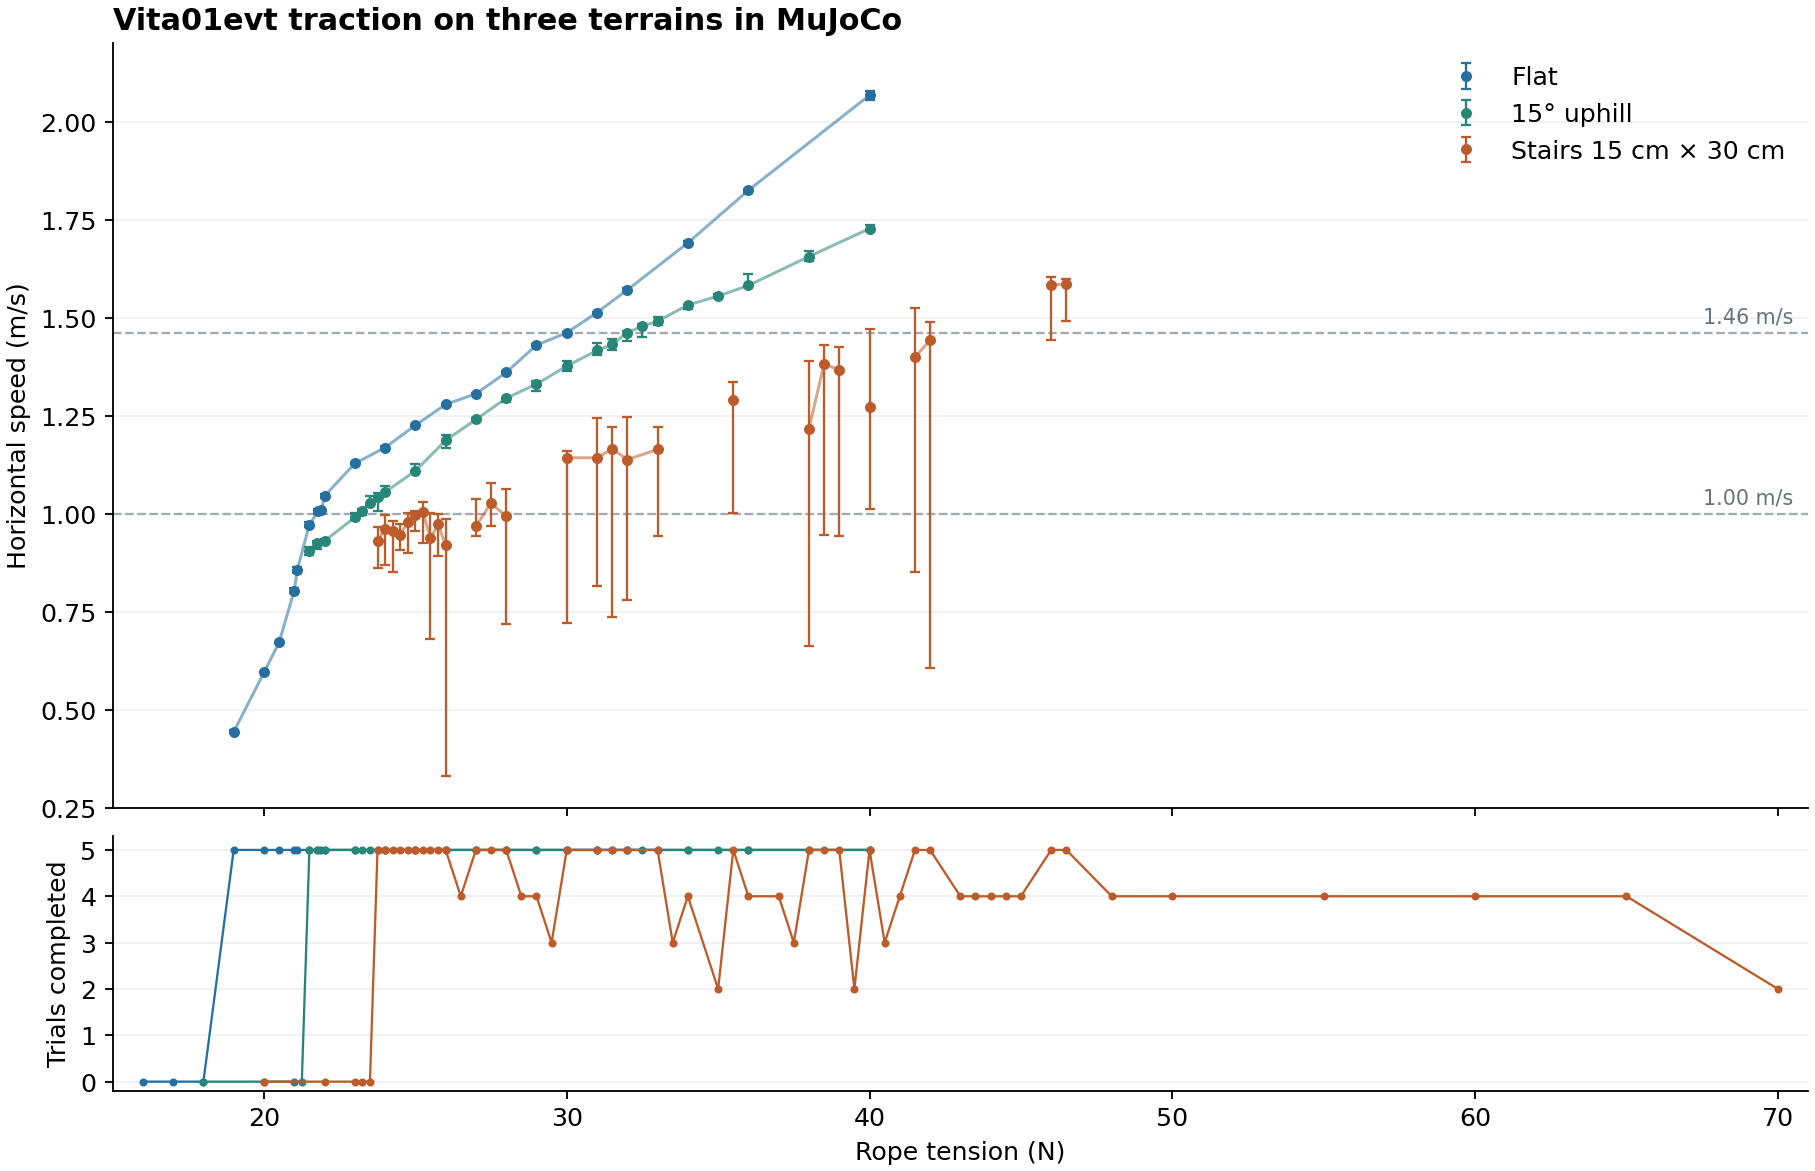
\includegraphics[width=0.95\linewidth]{figures/01_force_speed.png}
\captionof{figure}{拉力、水平速度与完成次数。上图绘制五次均完成的档位，圆点为中位数，误差棒为最小值至最大值。}
\end{minipage}

\clearpage
\section{固定绳角下坡度与级高的牵引力曲线}

设楼梯级高为 \(h\)、踏面深度为 \(d\)，等效坡角为
\(\theta=\arctan(h/d)\)。踏面固定为 \(30\unit{cm}\) 时，
\(15^\circ\) 斜坡对应 \(8.04\unit{cm}\) 级高，\(15\unit{cm}\) 级高对应 \(26.6^\circ\)。

本实验共 810 次，三种地形的绳角均固定为 \(33.4^\circ\)。
每组取五次均完成、且每次平均水平速度均至少为 \(1.0\unit{m/s}\) 的最低实测拉力档位。
实验一按约 \(1.0\unit{m/s}\) 匹配速度，并按各地形设置绳角，两张表采用各自的平地基线。

\begin{minipage}{\linewidth}
\centering
\captionof{table}{同一等效坡角下五次均达到 \(1.0\unit{m/s}\) 的最低实测拉力}
\begin{tabular}{r r r c}
\toprule
级高 \(\mathrm{(cm)}\) & 等效坡角 \((^\circ)\) & 连续斜坡 \(\mathrm{(N)}\) & 楼梯 \(\mathrm{(N)}\) \\
\midrule
0 & 0.0 & 22.5 & 22.5 \\
3 & 5.7 & 23.5 & 23.0 \\
6 & 11.3 & 23.5 & 23.0 \\
8.04 & 15.0 & 23.5 & 22.5 \\
9 & 16.7 & 24.0 & 23.0 \\
12 & 21.8 & 25.5 & 22.5 \\
15 & 26.6 & 29.0 & 29.0 \\
18 & 31.0 & 31.0 & \(48\unit{N}\) 内未达标 \\
\bottomrule
\end{tabular}
\end{minipage}

连续斜坡从约 \(15^\circ\) 起，达标拉力随坡角增加。
楼梯在 \(3\)--\(12\unit{cm}\) 内集中于 \(22.5\)--\(23.0\unit{N}\)，到 \(15\unit{cm}\) 升至 \(29\unit{N}\)，
该档速度中位数为 \(1.22\unit{m/s}\)。级高达到 \(18\unit{cm}\) 后，在测过的档位上没有一次达到 \(1.0\unit{m/s}\)。
平均坡角相同的两种地形可出现不同的牵引响应。

\begin{minipage}{\linewidth}
\centering
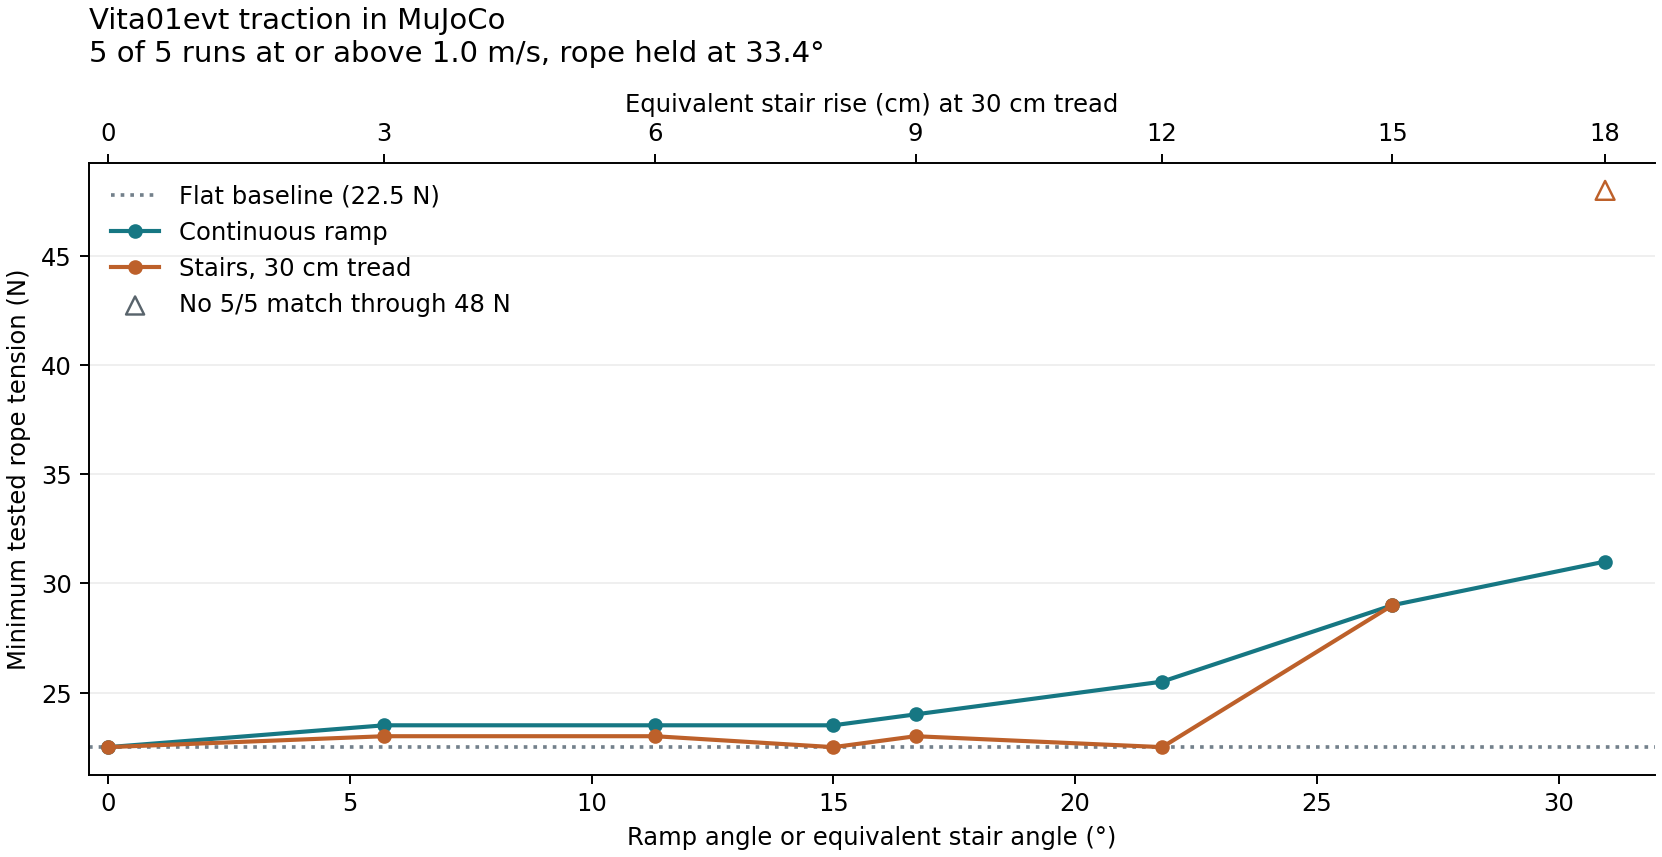
\includegraphics[width=0.95\linewidth]{figures/02_geometry_force.png}
\captionof{figure}{达标拉力随等效坡角和级高的变化。空心三角位于楼梯最后测试的 \(48\unit{N}\) 档。}
\end{minipage}
\clearpage
\section{固定相对机身角的地形对照}
\label{sec:body-angle}

实验三对平地、\(15^\circ\) 斜坡和级高 \(15\unit{cm}\)、踏面深度 \(30\unit{cm}\) 的楼梯进行交叉对照，共 1270 次。
各次试验固定绳张力，水平牵引指向沿世界系 \(+x\)。
每个仿真步用机身前向轴在世界 \(x\)--\(z\) 平面上的仰角 \(\beta(t)\) 更新世界系绳角
\(\alpha(t)=\gamma+\beta(t)\)，从而让矢状面内相对机身的绳角 \(\gamma\) 保持在设定值。

\begin{minipage}{\linewidth}
\centering
\captionof{table}{五次均完成且达到 \(1.0\unit{m/s}\) 的最低实测绳张力}
\label{tab:body-angle}
\begin{tabular}{l r r r}
\toprule
地形 & \(\gamma=16.9^\circ\) & \(\gamma=18.4^\circ\) & \(\gamma=24.4^\circ\) \\
\midrule
平地 & \(22.0\unit{N}\) & \(22.0\unit{N}\) & \(22.0\unit{N}\) \\
\(15^\circ\) 斜坡 & \(23.0\unit{N}\) & \(23.5\unit{N}\) & \(23.5\unit{N}\) \\
\(15\unit{cm}\) 楼梯 & \(24.5\unit{N}\) & \(25.0\unit{N}\) & \(32.0\unit{N}\) \\
\bottomrule
\end{tabular}
\end{minipage}

在三个相对角下，\(15^\circ\) 斜坡比平地仅多 \(1\)--\(1.5\unit{N}\)（约 \(5\%\)--\(7\%\)）。
固定 \(16.9^\circ\) 从平地换到楼梯多 \(2.5\unit{N}\)，在同一楼梯上把相对角增至 \(24.4^\circ\) 又多 \(7.5\unit{N}\)。
这反映了楼梯对较大相对角更敏感。

固定相对角时，世界系绳角随俯仰而变。表中跨地形的差值反映了这一控制条件下，重力、地面接触和牵引方向共同作用的结果。

\begin{minipage}{\linewidth}
\centering
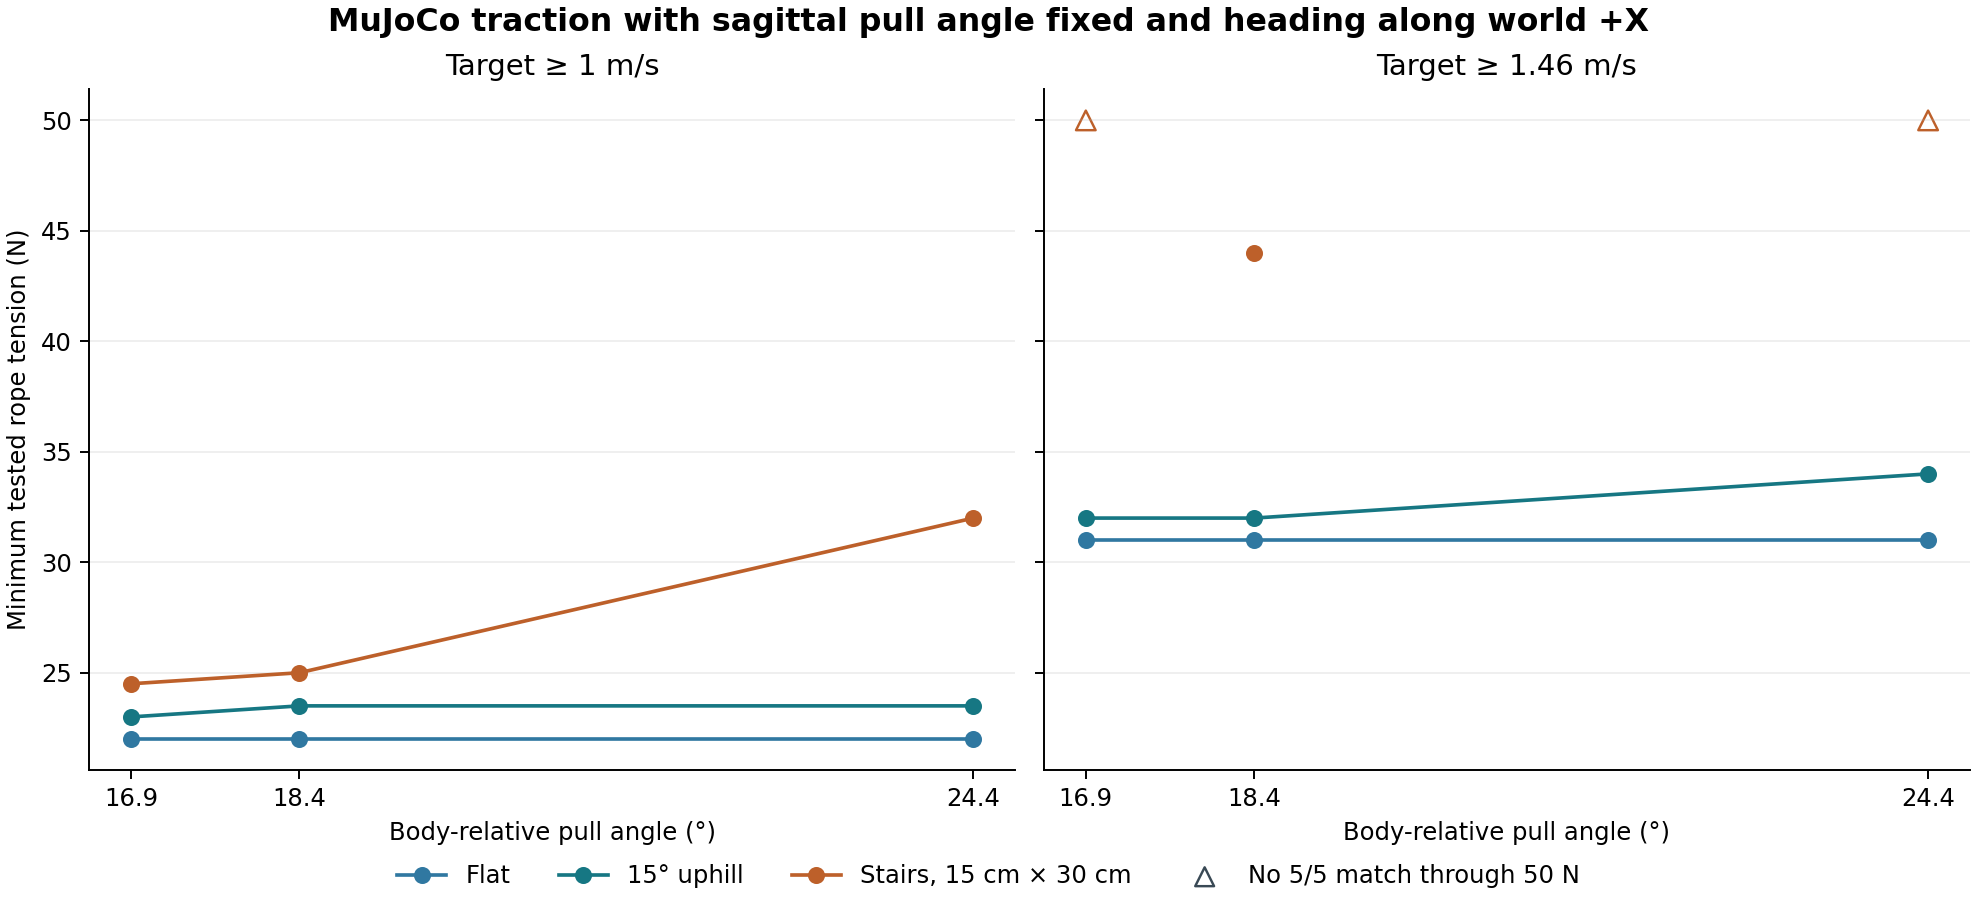
\includegraphics[width=0.98\linewidth]{figures/03_body_angle_vs_terrain.png}
\captionof{figure}{不同相对机身角下的达标张力。空心三角表示扫到 \(50\unit{N}\) 仍未五次均达标。}
\end{minipage}

目标提高到 \(1.46\unit{m/s}\) 时，平地需 \(31\unit{N}\)，斜坡需 \(32\)--\(34\unit{N}\)。
楼梯在相对角 \(18.4^\circ\) 时用 \(44\unit{N}\) 五次均达标，其余两个角度在测试范围内均未五次全过。
\end{document}

